\section{\textbf{Introduction}}

\subsection{\textbf{Compositional Explanations}}

Understanding what individual neurons in a neural network represent is a central challenge in interpretability. \cite{compex} proposed a method for explaining neurons by identifying compositional logical concepts that approximate their behavior. Their work extended prior approaches like Network Dissection, which used atomic labels (e.g., "water," "car"), by allowing explanations to be compositions of concepts using logical operators like \texttt{AND}, \texttt{OR}, and \texttt{NOT}. This provides a more precise and expressive way to characterize the complex abstractions learned by neurons, showing, for example, that a neuron might fire for \texttt{"water" AND NOT "blue"}.

\subsection{\textbf{Encoded Absences}}

Building on Compositional Explanations \cite{compex}, "what is missing" \cite{whatismissing} found that specific neurons are consistently suppressed by the least-activating patches in an image. They measured this "absence effect" as the gap between activation from a random patch and activation from a least-activating patch, suggesting that neural networks actively encode negative information. This phenomenon, if real, has significant implications for interpretability: it implies that neurons do not simply detect features but also represent their absence — a form of logical \texttt{NOT} that \cite{compex} had already identified as a compositional operator.

\subsection{\textbf{Pruning and Optimal Brain Damage}}

Another line of research has focused on removing information from neural networks. Pruning, the practice of deleting unimportant connections or parameters to create more efficient models, has a long history in deep learning, dating back to Optimal Brain Damage (OBD) \cite{optimalbraindamage}, which proposed a principled approach to removing parameters while preserving function. More recent work has explored various pruning strategies, from unstructured pruning (removing individual weights) to structured pruning (removing entire filters or channels).

However, pruning is typically evaluated solely on accuracy preservation. Its impact on the interpretability of neural representations — whether the circuits we identify survive compression — remains largely \textit{unexplored}. This raises a critical question: \textbf{if we prune a network, do the "encoded absences" survive?} Or are they fragile artifacts that disappear when the network is compressed? Our work addresses this by stress-testing the absence phenomenon under various pruning strategies and sparsity levels.

\subsection{\textbf{The Dead Salmon of AI Interpretability}}

A growing body of work has sounded a note of caution for interpretability research. \cite{deadsalmon} identify what they call the "dead salmon" problem in AI interpretability. This refers to the famous neuroscience study where a dead Atlantic salmon placed in an fMRI scanner showed statistically significant "brain activity" due to a failure to correct for multiple comparisons. The lesson is that statistical artifacts can produce compelling, plausible-looking results from dead systems.

The dead salmon problem is not isolated. In AI, methods like feature attribution, probing, and causal analysis have been shown to produce seemingly meaningful explanations for randomly initialized neural networks — networks with no genuine representations to explain. The key concern is that findings in interpretability may be vulnerable to similar false discoveries unless they are subjected to rigorous testing against explicit and meaningful alternative hypotheses, with their statistical uncertainty properly quantified. see spurious correlations \footnote{https://tylervigen.com/spurious-correlations} for more.

\subsection{\textbf{Our Contribution}}

Our work sits at the intersection of these two lines of inquiry. We take the "encoded absence" phenomenon \cite{whatismissing} and subject it to a \textit{sanity check} in the spirit of the "dead salmon" critique \cite{deadsalmon}. Specifically, we stress-test the phenomenon by subjecting neural networks to pruning inspired by Optimal Brain Damage"s principle of removing parameters while preserving function \cite{optimalbraindamage} — which allows us to degrade network functionality while observing whether the absence effect persists.

We ask:

\begin{enumerate}
\item \textbf{Does the absence effect survive pruning?} Or is it a fragile artifact of over-parameterization?
\item \textbf{Do different pruning strategies preserve or destroy it differently?} If so, what does this tell us about the nature of the phenomenon?
\item When the effect appears to strengthen under pruning, is this genuine robustness or a statistical artifact?
\end{enumerate}

By doing so, we aim to determine whether "encoded absences" are a genuine, robust representational strategy \textit{or just another dead salmon of AI interpretability}.

\section{\textbf{Prior Works}}

\subsection{\textbf{Compositional Explanations of Neurons}}

Understanding what individual neurons represent is a central challenge in interpretability. Early work on \textbf{Network Dissection} introduced a quantitative framework to measure the interpretability of CNN units by aligning their activations with a comprehensive set of human-labeled concepts. While powerful, this approach was limited to \textbf{atomic labels} (e.g., "water", "car," "fur") — it could only describe neurons in terms of single, pre-defined concepts \cite{netdissec}.

Mu and Andreas extended this paradigm by proposing \textbf{compositional explanations} of neurons. Instead of atomic labels, they identified \textbf{logical compositions of concepts} — using operators like AND, OR, and NOT — that closely approximate neuron behavior\}. Their approach uses a beam search procedure to discover logical forms that maximize Intersection over Union (IoU) with neuron activation masks, allowing formulas up to a maximum length \cite{compex}. For example, a neuron might fire for "\texttt{water AND (NOT blue)}" or "\texttt{car OR truck}".


This allowed for more precise and expressive characterizations of the abstractions learned by neurons. Their analysis revealed that many vision neurons learn highly abstract but semantically coherent visual 
concepts, while other
 \textbf{polysemantic neurons} detect multiple unrelated features. They further demonstrated that vision neurons detecting human-interpretable concepts are positively correlated with task performance \cite{compex}.

\subsection{\textbf{Encoded Absences}}

Building on the idea of logical \texttt{NOT} as a compositional operator, Hesse et al. made a novel claim: neurons can encode not only the \textbf{presence} of features but also their \textbf{absence}. Their paper, "What is Missing? Explaining Neurons Activated by Absent Concepts" found that specific neurons are consistently suppressed by the least-activating patches in an image \cite{whatismissing}.

The authors observed that mainstream XAI methods, when applied in their standard form, struggle to reveal these "encoded absences". To address this, they proposed two simple extensions to attribution and feature visualization techniques that uncover these missing concepts.  Their lay summary captures the intuition: \textit{"models can also use information that is missing in the image... a model predicting "Irish Setter" may rely on not seeing concepts that are typical for other dog breeds"} \cite{whatismissing}.

Across their experiments, they showed how \texttt{ImageNet} \cite{imagenet} models exploit encoded absences, and debiasing can be improved when considering them. Importantly, they measured the "absence effect" as the gap between activation from a random patch and activation from a least-activating patch, using a sliding-window approach to find the patches that most strongly suppress neuron activations. This phenomenon, if real, has significant implications for interpretability: it implies that neurons do not simply detect features but also represent their absence — a form of logical \texttt{NOT} that Mu and Andreas \cite{compex} had already identified as a compositional operator.

\subsection{\textbf{Gap in the Literature}}

To date, no work has tested whether "encoded absences" survive neural network pruning, nor whether the phenomenon is robust or fragile when the network is compressed. Our work bridges model compression and interpretability by stress-testing the absence effect across multiple pruning strategies and sparsity levels, serving as a sanity check in the spirit of the dead salmon critique.

\section{\textbf{Methodology}}

\subsection{\textbf{Overview}}

Our experimental pipeline consists of 3 main stages:

\begin{enumerate}
\item we establish a baseline by evaluating the "absence effect" in a dense (unpruned) model, replicating the procedure from Hesse et al. \cite{whatismissing}.
\item we apply various pruning strategies to the model at increasing sparsity levels.
\item we re-evaluate the absence effect in each pruned model, comparing the results against the dense baseline to assess whether the phenomenon survives compression.
\end{enumerate}

\subsection{\textbf{Model and Dataset}}

We use a \texttt{ResNet-50} \cite{resnet} architecture pretrained on \texttt{ImageNet-1K} \cite{imagenet}. This choice is motivated by two factors: (1) it is the same architecture and dataset used in the original "What is Missing?" paper, ensuring comparability of results, and (2) it is a widely studied benchmark model, making our findings relevant to the broader interpretability and pruning communities.

The pretrained model achieves a top-1 accuracy of \textbf{79.2\%} and top-5 accuracy of \textbf{94.7\%} on the ImageNet validation set, consistent with reported performance for standard \texttt{ResNet-50}.

\subsection{\textbf{Measuring the Absence Effect}}

Following Hesse et al. \cite{whatismissing}, we measure the absence effect using the following procedure:

\subsubsection{\textbf{Finding Least-Activating Patches}}

For each channel/neuron in the model, we search for the \textbf{least-activating 64 \(\times\) 64  pixel patch} using a \textit{sliding-window approach} with a stride of 16 pixels. This process scans the entire image, extracting patches at every possible window position and recording the resulting neuron activation. We then identify the patches that produce the \textbf{lowest} activation values.

\subsubsection{\textbf{Computing Activation Metrics}}

For each pruning configuration, we compute the following metrics:

\begin{itemize}
\item \textbf{Global L1  (All)} — *Unstructured, global:* All layers are pruned simultaneously using a single threshold across the entire network.
\item \textbf{Local L1  (All)} — *Unstructured, local:* Each layer is pruned independently to achieve the same target sparsity per layer.
\item \textbf{Local L1  (Conv2)} — *Unstructured, local:* Only \texttt{conv2} layers are pruned; all other layers remain intact.
\end{itemize}

A larger \textbf{Absence Gap} indicates a stronger "absence detection" effect: the neuron is actively suppressed by the least-activating patch. A large \textbf{Dynamic Range} in pruned models may indicate unstable activations, potentially signaling network collapse rather than genuine representational shifts.

\subsection{\textbf{Pruning Methods}}

We apply 3 pruning strategies to stress-test the absence effect:

For each method, we evaluate sparsity levels ranging from 0\% (dense baseline) to 95\%, with intermediate levels at 30\%, 60\%, 70\%, 85\%, and 90\% where applicable.

\subsection{\textbf{Implementation Details}}

Our experiments are implemented in \textbf{PyTorch} \cite{pytorch}. We forked the official code repository for the "What is Missing?" \footnote{https://github.com/visinf/what-is-missing} paper and extended it to support pruning and evaluation of pruned models. All pruning is performed using PyTorch"s built-in \texttt{torch.nn.utils.prune} module, which provides implementations of \(L_1\) magnitude pruning for both global and local strategies. The code and full results are available at: https://github.com/hamidb80/pruning-absent

\subsection{\textbf{Evaluation Protocol}}

For each pruning configuration (method  \(\times\)  sparsity level), we:

\begin{enumerate}
\item \textbf{Prune} the pretrained model to the target sparsity.
\item \textbf{Measure accuracy} on the ImageNet \cite{imagenet} validation set.
\item \textbf{Compute absence metrics} (Random, Most, Least, Absence Gap, Dynamic Range) using the sliding-window procedure.
\item \textbf{Compare} against the dense baseline to determine whether the absence effect is preserved, weakened, or destroyed.
\end{enumerate}

We report mean activation values with standard deviations, following the protocol established in the original paper.

\section{\textbf{Results}}

\begin{figure*}[!htb]
\centering
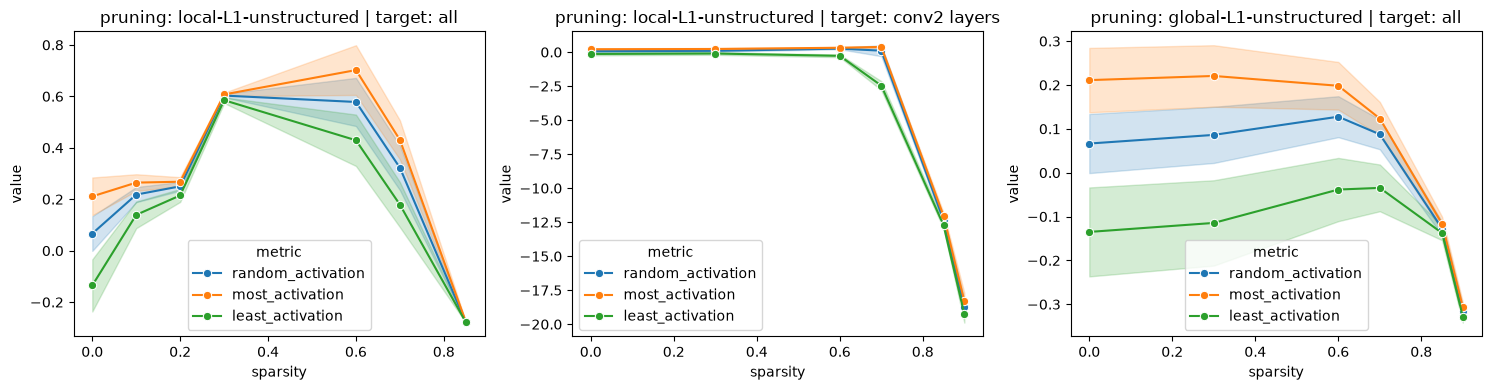
\includegraphics[width=15.0cm,keepaspectratio]{pruning-absense-fig-all-results.png}
\caption{\begin{small}Comparison of absence gap across pruning methods and sparsity levels\end{small}}
\label{fig:cmp}
\end{figure*}

\begin{table*}[!htb]
\centering
\footnotesize
\begin{tabular}{l l c c c c c c c}
\toprule
\textbf{Method} & \textbf{Target} & \textbf{Sparsity} & \textbf{Top-1} & \textbf{Top-3} & \textbf{Top-5} & \textbf{Random} & \textbf{Most} & \textbf{Least} \\
\midrule
local-L1-unstructured & all & 0.00 & 0.79214 & 0.91956 & 0.94738 & $0.0665\pm0.0674$ & $0.2111\pm0.0734$ & $-0.1350\pm0.1014$ \\
local-L1-unstructured & all & 0.10 & 0.18876 & 0.29246 & 0.33684 & $0.2180\pm0.0295$ & $0.2646\pm0.0326$ & $0.1393\pm0.0518$ \\
local-L1-unstructured & all & 0.20 & 0.00176 & 0.00484 & 0.00706 & $0.2502\pm0.0171$ & $0.2681\pm0.0177$ & $0.2148\pm0.0252$ \\
local-L1-unstructured & all & 0.30 & 0.00128 & 0.00336 & 0.00512 & $0.6030\pm0.0068$ & $0.6074\pm0.0069$ & $0.5850\pm0.0111$ \\
local-L1-unstructured & all & 0.60 & 0.00072 & 0.00256 & 0.00504 & $0.5781\pm0.0936$ & $0.7021\pm0.0967$ & $0.4292\pm0.0999$ \\
local-L1-unstructured & all & 0.70 & 0.00152 & 0.00368 & 0.00536 & $0.3223\pm0.0871$ & $0.4307\pm0.0761$ & $0.1790\pm0.0876$ \\
local-L1-unstructured & all & 0.85 & 0.00000 & 0.00000 & 0.00000 & $-0.2776\pm0.0015$ & $-0.2764\pm0.0014$ & $-0.2781\pm0.0016$ \\
\midrule
local-L1-unstructured & conv2 layers & 0.00 & 0.79214 & 0.91956 & 0.94738 & $0.0665\pm0.0674$ & $0.2111\pm0.0734$ & $-0.1350\pm0.1014$ \\
local-L1-unstructured & conv2 layers & 0.30 & 0.77926 & 0.91134 & 0.94036 & $0.0950\pm0.0641$ & $0.2301\pm0.0699$ & $-0.1028\pm0.0964$ \\
local-L1-unstructured & conv2 layers & 0.60 & 0.29940 & 0.43966 & 0.49628 & $0.2583\pm0.0486$ & $0.3210\pm0.0498$ & $-0.2739\pm0.0989$ \\
local-L1-unstructured & conv2 layers & 0.70 & 0.00376 & 0.00890 & 0.01246 & $0.1060\pm0.4023$ & $0.3818\pm0.0616$ & $-2.4629\pm0.3291$ \\
local-L1-unstructured & conv2 layers & 0.85 & 0.00100 & 0.00300 & 0.00500 & $-12.3438\pm0.2505$ & $-12.0391\pm0.2402$ & $-12.7266\pm0.2529$ \\
local-L1-unstructured & conv2 layers & 0.90 & 0.00100 & 0.00300 & 0.00500 & $-18.7500\pm0.6152$ & $-18.2969\pm0.6108$ & $-19.2500\pm0.6313$ \\
local-L1-unstructured & conv2 layers & 0.93 & 0.00000 & 0.00000 & 0.00000 & $-19.5156\pm0.3381$ & $-19.1875\pm0.3359$ & $-19.8750\pm0.3650$ \\
local-L1-unstructured & conv2 layers & 0.95 & 0.00000 & 0.00000 & 0.00000 & $-17.6094\pm0.2104$ & $-17.4531\pm0.2131$ & $-17.7969\pm0.2153$ \\
\midrule
global-L1-unstructured & all & 0.00 & 0.79214 & 0.91956 & 0.94738 & $0.0665\pm0.0674$ & $0.2111\pm0.0734$ & $-0.1350\pm0.1014$ \\
global-L1-unstructured & all & 0.30 & 0.78812 & 0.91752 & 0.94570 & $0.0862\pm0.0640$ & $0.2206\pm0.0701$ & $-0.1145\pm0.0973$ \\
global-L1-unstructured & all & 0.60 & 0.72290 & 0.86920 & 0.90496 & $0.1277\pm0.0467$ & $0.1982\pm0.0543$ & $-0.0384\pm0.0721$ \\
global-L1-unstructured & all & 0.70 & 0.59712 & 0.76018 & 0.80650 & $0.0875\pm0.0341$ & $0.1235\pm0.0379$ & $-0.0346\pm0.0533$ \\
global-L1-unstructured & all & 0.85 & 0.01184 & 0.04368 & 0.06712 & $-0.1273\pm0.0156$ & $-0.1165\pm0.0162$ & $-0.1375\pm0.0165$ \\
global-L1-unstructured & all & 0.90 & 0.00100 & 0.00436 & 0.00662 & $-0.3150\pm0.0117$ & $-0.3069\pm0.0117$ & $-0.3281\pm0.0137$ \\
\bottomrule
\end{tabular}
\caption{Complete experimental results for all pruning configurations. Accuracy (Top-1, Top-3, Top-5) and activation metrics (Random, Most, Least) are reported with standard deviations where applicable.}
\label{tab:all}
\end{table*}


We should also note that changing the random seed value and dataset split makes the numbers change remarkably. it means that if you don't run our experiments with our setup (seed=0 and dataset split of  \(1/4\)  you may get completely different values) but the overall behavior remains the same.

\section{\textbf{Discussion}}

based on the results in Fig. \ref{fig:cmp} and Table. \ref{tab:all}, we can conclude several statements:

\subsection{\textbf{The metric is quite unreliable}}

for \texttt{local-L1-unstructured} , (where accuracy collapsed immediately) the activations collapse to a single value between pruning percent of 20\% and 30\% but then the difference grows after 30\%. the \textit{standard deviation} also grows.

\subsection{\textbf{Standard deviation is not informative}}

This may trigger us to blindly conclude that if the standard deviation may show the health and validity of the metric; but considering \texttt{local-L1-unstructured} at sparsity 20\% and \texttt{global-L1-unstructured} at sparsity 60\% (with top-1 of 72\% vs 0\% and top-5 of 90\% vs 0\%), it's quite visible that the standard deviation value does not give much information about absence and health of the network.

\section{\textbf{Future Work}}

Our findings suggest several promising directions for future research:

\begin{enumerate}
\item extending our analysis to other pruning algorithms — such as structured pruning, \texttt{SlimPruner}, \texttt{L1FilterPruner}, and the Lottery Ticket Hypothesis \cite{lottery} — would reveal whether the absence effect survives different forms of sparsity.
\item evaluating other architectures, particularly Vision Transformers \cite{vit}, would help determine whether our findings generalize beyond CNNs.
\end{enumerate}

\section{\textbf{Conclusion}}

Hesse et al. \cite{whatismissing} provide compelling visual evidence for their claim of encoded absences in neural networks. Their \textit{Figure 6} illustrates, for channels identified as important for specific classes, both the most activating patches (positive potential) and the least activating patches (encoded absences). This visualization is particularly striking for fine-grained classification tasks, such as distinguishing between closely related dog breeds, where the absence of patterns from related species appears to be actively leveraged by the network. The authors argue that this mechanism allows the model to disambiguate between visually similar classes by relying not only on what is present in the image, but also on what is conspicuously missing.

Yet, our stress-test through pruning reveals that this absence effect — while robust when accuracy is maintained — exhibits troubling behavior when the network is damaged. This pattern suggests that the absence effect, while real in healthy networks, is not an invariant property of the architecture but rather a phenomenon that appears to \textbf{correlate} with network accuracy, not a causally robust feature of the architecture itself.

\begin{acks}

We acknowledge the following resources and tools that made this work possible:

\begin{itemize}
\item \textbf{Computational resources:} The \textit{Kaggle} platform provided the cloud‑based computing environment used for our experiments.
\item \textbf{Writing and formatting:} Tangent Notes  \footnote{https://github.com/suchnsuch/Tangent} was employed to write the manuscript in Markdown.
\item \textbf{Conversion to LaTeX:} The Markdown file was transformed into a TeX document using a simple, hand‑written compiler  \footnote{https://github.com/hamidb80/damn‑hackable‑markdown‑parser‑tex} .
\end{itemize}

\end{acks}